\section{Лекция 8}

\subsection{Кривые Пеано}

\begin{definition}
    Кривая в топологическом пространстве $X$ --- это непрерывное отображение $\gamma: [0,1] \to X$.
\end{definition}

\begin{definition}
    Кривая Пеано --- общее название для непрерывных сюръекций $\gamma: I \to I^2$, где $I = [0,1]$, т.е. для кривых, заполняющих квадрат.
\end{definition}

\begin{theorem}[Кривая Пеано]
    Кривая Пеано существует.
\end{theorem}

\begin{nota_bene}
    Первыми построили примеры кривых Пеано сам Джузеппе Пеано и Давид Гильберт. Оба построения были рекурсивными и состояли в последовательном делении квадрата на несколько частей с последующим определением поведения кривой в каждой части. В построении Пеано квадрат делился на 9 частей, а в построении Гильберта --- на 4. Мы построим кривую иным способом, сначала отобразив отрезок $[0, 1]$ непрерывно и сюръективно в треугольник, а затем отобразив треугольник в квадрат. 
\end{nota_bene}

% \begin{center}
%     \begin{tikzpicture}
%         \draw (0,0) -- (2, 0) -- (2, 3);
%     \end{tikzpicture}
% \end{center}

\begin{proof}
    Мы построим кривую в два этапа, сначала отобразив отрезок [0, 1] непрерывно и сюръективно в треугольник, а затем отобразив треугольник в квадрат.
    \begin{center}
        \begin{tikzpicture}
            \text{0-ой шаг} \draw (0,0) -- (1,0) -- (0, 1) -- (0,0);
        \end{tikzpicture}
        
        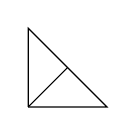
\begin{tikzpicture}
            \draw (0,0) -- (1,0) -- (0, 1) -- (0,0);
            \draw (0,0) -- (0.5, 0.5);
        \end{tikzpicture}

        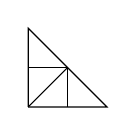
\begin{tikzpicture}
            \draw (0,0) -- (1,0) -- (0, 1) -- (0,0);
            \draw (0,0) -- (0.5, 0.5);
            \draw (0,0.5) -- (0.5, 0.5);
            \draw (0.5,0) -- (0.5, 0.5);
        \end{tikzpicture}
    \end{center}
    
    % \begin{center}
    %     \begin{tikzpicture}
    %         \draw (0,0) -- (1,0);
    %     \end{tikzpicture}
    % \end{center}

    Пусть $\Delta$ --- прямоугольний равнобедренный треугольник с катетами длины $1$ и $I = [0,1]$. На первом шаге разобъём исходные треугольник и отрезок пополам, а на каждом следующем шаге будем разбивать пополам полученные ранее подтреугольники и подотрезки. На n-ом шаге будем иметь $2^n$ треугольников и отрезок, разбитый на столько же частей. На каждом шаге будем нумеровать треугольники и части отрезка двоичными кодами. 
    
    Будем иметь следующую нумерацию: $\Delta_{i_1 \ldots i_n}$ и $I_{i_1 \ldots i_n}$. При этом: $I = I_0 \cup I_1 = I_{00} \cup I_{01} \cup I_{10} \cup I_{11} = ... = \bigcup_{i_1, \ldots, i_n \in \cbr{0,1}} I_{i_1 \ldots i_n}$. То же для $\Delta$.
    Определим соседние элементы как подтреугольники, у которых есть общая сторона (для разбиения треугольников) и подотрезки, у которых есть общая точка (для разбиения отрезка).
    Так же мы имеем цепочку вложенных отрезков (треугольников).

    \[
        I_{i_1} \supset I_{i_1 i_2} \supset I_{i_1 i_2 i_3} \supset \ldots
    \]
    \[
        \Delta_{i_1} \supset \Delta_{i_1 i_2} \supset \Delta_{i_1 i_2 i_3} \supset \ldots
    \]

    Из элементарных геометрических соображений можем найти значения диаметров этих множеств (т.е. длины наибольших отрезков, лежащих в множествах: для отрезков это длины самих отрезков, а для треугольников --- длины их гипотенуз, т.к. все треугольники в разбиении прямоугольные и равнобедренные). Т.о.:
    Видим, что диаметр множеств стремится к $0$ с ростом $n$.

    \[
        \diam(I_{i_1 i_2 \ldots i_n}) = \br{\frac{1}{2}}^n
    \]
    \[
        \diam(\Delta_{i_1 \ldots i_n}) = \br{\frac{1}{\sqrt{2}}}^{n - 1}
    \]

    Очевидно, что все подтреугольники и подотрезки являются компактами (т.к. они являются замкнутыми и ограниченными подмножествами полного метрического пространства $\R^2$).
    Начнём строить отображение $f: I \to \Delta$ пошагово. \textbf{Приведём сначала \underline{неполное построение}, в котором могут возникнуть неоднозначности, а затем уточним его.}

    Рассмотрим $t \in I = [0, 1]$. Существует последовательность вложенных отрезков, стягивающаяся к $t$:
    \[
        I_{i_1} \supset I_{i_1 i_2} \supset I_{i_1 i_2 i_3} \supset \ldots \ni t.
    \]
    Т.к. $t$ может лежать на границе отрезков, то последовательность может быть определена неоднозначно.
    Возьмем последовательность треугольников с теми же индексами. Это будет последовательность вложенных компактов, причём их диаметры стремятся к $0$. Т.о. пересечение этих треугольников будет состоять из одной точки, и эту единственную точку мы положим значением $f(t)$.

    У этого рассуждения есть недостаток: $t$ может принадлежать двум множествам $I_{i_1 \ldots i_n}$ и $I_{j_1 \ldots j_n}$, а значит, $f(t)$ может быть определено неоднозначно. Дополним рассуждения, убрав неоднозначность:
    Рассмотрим новое множество $J_{i_1 \ldots i_n}$, соответствующее точке $t \in I$, такое что: 
    \[
        J_{i_1 \ldots i_n} = 
        \begin{cases}
            I_{i_1 \ldots i_n}, & \text{ если $t$ не лежит на границе $I_{i_1 \ldots i_n}$}, \\
            I_{i_1 \ldots i_n} \cup I_{j_1 \ldots j_n}, & \text{ если $t$ лежит на границе $I_{i_1 \ldots i_n}$ и $I_{j_1 \ldots j_n}$}.
        \end{cases}
    \]
    Также определим соответствующее множество 
    \[
        P_n(t) =
        \begin{cases}
            \Delta_{i_1 \ldots i_n}, & \text{ если $t$ не лежит на границе $I_{i_1 \ldots i_n}$}, \\
            \Delta_{i_1 \ldots i_n} \cup \Delta_{j_1 \ldots j_n}, & \text{ если $t$ лежит на границе $I_{i_1 \ldots i_n}$ и $I_{j_1 \ldots j_n}$}.
        \end{cases}
    \]
    Получим новую последовательность компактов:
    \[
        P_1(t) \supset P_2(t) \supset \ldots
    \]

    \begin{statement}
        \[
            \diam P_n(t) \leq \br{\frac{1}{\sqrt{2}}}^{n - 2}
        \]
    \end{statement}
    Значит, $P_n(t)$ образуют последовательность вложенных компактов, причём их диаметры стремятся к $0$. Значит, их пересечение состоит из одной точки, и эту точку мы положим значением $f(t)$. При данном построении неоднозначности уже не возникает, а значит, получено корректное отображение $f: I \to \Delta$.

    Докажем, что $f$ сюръективно. 
    Рассмотрим точку $x_0$ из треугольника $\Delta$. Эта точка будет лежать в некоторой последовательности вложенных треугольников $\Delta_{i_1} \supset \Delta_{i_1 i_2} \supset \Delta_{i_1 i_2 i_3} \supset \ldots$. Рассмотрим последовательность подотрезков с теми же индексами: в пересечении этих подотрезков будет лежать одна единственная точка $t_0$. Остается доказать, что это точка --- прообраз точки $x_0$. По $t_0$ однозначно строится последовательность $\cbr{P_n(t_0)}$, сходящаяся к одной точке $y \in \Delta$. Но $\forall n: \ P_n(t_0)$ содержат $\Delta_{i_1 \ldots i_n}$, значит, последовательность вложенных отрезков $\cbr{\Delta_{i_1 \ldots i_n}}$ также сходится к точке $y$. Но тогда: $x_0 = y$, т.е. $t_0$ является прообразом точки $x_0$, а значит, отображение $f$ сюръективно.

    Докажем, что $f$ непрерывно.
    Рассмотрим точку $x_0$ из треугольника $\Delta$. Покажем, что $\forall \, \veps > 0 \ \exists \, \delta > 0: \ f(U_{\delta}(t_0)) \subset O_{\veps}(x_0)$, где $f(t_0) = x_0$. Т.к. $\diam P_n(t_0) \longrightarrow 0$ при $n \longrightarrow \infty$, то $\exists N \in \N: \forall n > N: P_n(t_0) \subset O_{\veps}(x_0)$.
    
    Если $P_N(t_0)$ --- это один треугольник $\Delta_{i_1 \ldots i_N}$ начального разбиения, то рассмотрим соответствующий ему отрезок $I_{i_1 \ldots i_N}$, содержащий $t_0$, и положим значение $\delta$ равным наименьшему расстоянию от $t_0$ до концов отрезка $I_{i_1 \ldots i_N}$.
    Если $P_N(t_0)$ --- это объединение двух треугольников $\Delta_{i_1 \ldots i_N} \cup \Delta_{j_1 \ldots j_N}$ начального разбиения, то рассмотрим соответствующие им отрезки $I_{i_1 \ldots i_N}$ и $I_{j_1 \ldots j_N}$: $t_0$ лежит в их пересечении, т.е. является граничной точкой обоих отрезков. Положим в этом случае значение $\delta$ равным половине длины отрезка $I_{i_1 \ldots i_N}$.
    
    Т.о. получили $\delta = \delta(\veps)$, причём в силу оценки на диаметр множеств $P_n(t)$: $\forall t \in U_{\delta}(t_0) \, \forall n \in \N: P_n(t) \subset P_n(t_0)$, при этом $f(t) = \lim_{n \to \infty} P_n(t)$. Значит, $f(t) \in O_{\veps}(x_0) \ \forall t \in U_{\delta}(t_0)$, а значит, отображение $f$ непрерывно.

    Остаётся отобразить треугольник непрерывно и сюръективно на квадрат. Это будет сделано в следующем лекции.
\end{proof}

\begin{definition}
    Пусть $X$ --- топологическое пространство, $f_n: X \rightarrow \R$ --- последовательность функций.
    Говорят, что $f_n$ равномерно сходится к функции $f: X \to \R$ на $X$ и пишут $f_n \rightrightarrows f$, если для любого $\veps > 0$ существует $N \in \N$ такое, что для любого $n \geq N$ и для любого $x \in X$ выполняется $|f_n(x) - f(x)| < \veps$.
\end{definition}

\begin{theorem}
    Предел равномерно сходящейся последовательности непрерывных функций является непрерывной функцией.
\end{theorem}
\begin{proof}
    Доказательство теоремы остаётся читателю в качестве упражнения.
\end{proof}